\newpage
\subsection{Multiplexores}
Un multiplexor es un circuito combinacional que selecciona información binaria de una de muchas líneas de entrada y la envía a una sola línea de salida. La selección de una línea de entrada dada se controla con un conjunto de líneas de selección. Normalmente, hay $2^n$ líneas de entrada y $n$ líneas de selección cuyas combinaciones de bits determinan cuál entrada se selecciona.


\subsubsection{Multiplexor de 2 a 1}
Un multiplexor de $2$ líneas a $1$ conecta una de dos fuentes de un bit a un destino común. El circuito tiene dos líneas de entrada de datos, una línea de salida y una línea de selección $S$. Cuando $S=0$, se habilita la compuerta \texttt{AND} de arriba e $I_0$ cuenta con una trayectoria hacia la salida. Cuando $S=1$, la compuerta \texttt{AND} inferior está habilitada e $I_1$ tiene una trayectoria hacia la salida. El multiplexor actúa como un interruptor electrónico que selecciona una de dos fuentes. El diagrama de bloques de un multiplexor a veces se representa con un símbolo en forma de cuña. Esto sugiere visualmente cómo una fuente de datos, seleccionada de entre varias, se dirige a un solo destino. En los diagramas de bloques es común rotular los multiplexores como \texttt{MUX}.
\begin{figure}[h]
\centering
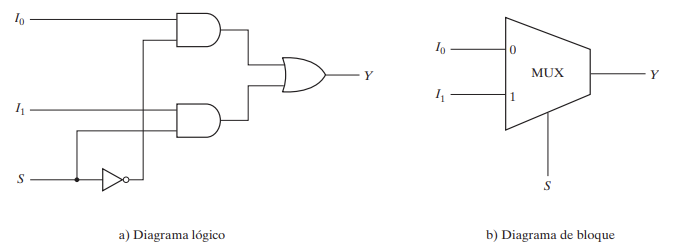
\includegraphics[scale=0.8]{img/mux2a1.png}
\caption{Multiplexor de 2 a 1}
\end{figure}

\subsubsection{Implementación de funciones lógicas con multiplexores}
Un examen del diagrama lógico de un multiplexor revela que básicamente es un decodificador con una compuerta \texttt{OR} incluida en la unidad. Los minitérminos de una función se generan en un multiplexor mediante el circuito asociado a las entradas de selección. Los minitérminos individuales se pueden seleccionar con las entradas de datos. Esto ofrece un método para implementar una función booleana de $n$ variables con un multiplexor que tiene $n$ entradas de selección y $2^n$ entradas de datos, una para cada minitérmino.

\begin{mdframed}[backgroundcolor=gray!10,linewidth=0pt]
Para implementar una función booleana de $n$ variables con un multiplexor que tiene $n-1$ entradas de selección. Las primeras $n-1$ variables de la función se conectan a las entradas de selección del multiplexor. La variable restante de la función se utiliza para las entradas de datos. Si denotamos esa variable con $z$, cada entrada de datos del multiplexor será, $z$, $z'$, $1$ o $0$.
\end{mdframed}

\newpage
\subsubsection{Ejemplo de Implementación}
Consideremos la función booleana de tres variables:

\begin{equation*}
    F(x,y,z) = \sum (1,2,6,7)
\end{equation*}

La función puede implementarse con un multiplexor de $4$ líneas a $1$. Las dos variables $x$ e $y$ se aplican a las líneas de selección en ese orden; $x$ se conecta la entrada $S_1$ y y se conecta a $S_0$. Los valores de las líneas de entrada de datos se deducen de la tabla de verdad de la función. Cuando $xy=00$, la salida $F$ es igual a $z$ porque $F=0$ cuando $z=0$ y $F=1$ cuando $z=1$. Esto requiere aplicar la variable $z$ a la entrada de datos $0$. El funcionamiento del multiplexor es tal que, cuando $xy=00$, la entrada de datos $0$ tiene una trayectoria hacia la salida y eso hace que $F$ sea igual a $z$. De forma similar, podemos determinar las entradas que deben recibir las líneas de datos $1$, $2$ y $3$, a partir del valor de $F$ cuando $xy=01$, $10$ y $11$, respectivamente.

\begin{figure}[h]
\centering
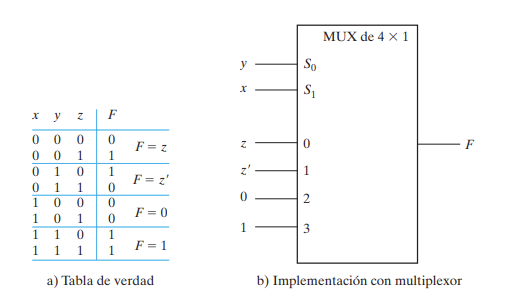
\includegraphics[scale=0.9]{img/ej1.png}
\caption{Implementación de una función booleana con un multiplexor}
\end{figure}